\newpage
\section{METHODOLOGY}
Image Super Resolution is a branch of Artificial Intelligence that deals with upscaling a Low-Resolution Image to High Resolution Image, filling in the missing pixels with the different techniques. There are other simpler methods to upscale images like Linear or Bi-cubic interpolation, but they do not generate any new information based on the environment and hence are not super useful to upscale an LR image. Deep Learning based methods require huge amounts of data so that the model is not overfitted, the dataset needs to contain an HR  LR version of the same image that are perfectly aligned to each other. We need to synthetically create LR images from HR images.
The ‘classical’ degradation model is the most used, which considers down-sampling, blurring, and noise:
 
$$I^{LR}= (I^{HR} \circledast k)\downarrow_s + n$$
where $\circledast$ represents a convolution operation, k is a kernel (typically a Gaussian blurring
kernel, but it can also represent other functions such as the Point Spread Function
(PSF)), n represents additive noise, and ↓s is a downscaling operation that is typically
assumed to be bicubic down-sampling with scale factor s.
SR aims to then reverse whichever degradation process is considered, to retrieve the original underlying high-fidelity image. We have implemented SSResNet and SRGAN till now. The methodology for them is explained below: 
\begin{enumerate}
    \item SRResNet: The SRResNet is a fully convolutional network designed for 4x super-resolution. It incorporates residual blocks with skip connections to increase the optimizability of the network despite its significant depth. The SRResNet is trained and used as a standalone network and provides a nice baseline for the SRGAN – for both comparison and initialization. We use the following architecture for this network.
    \begin{figure}[ht]
        \centering
        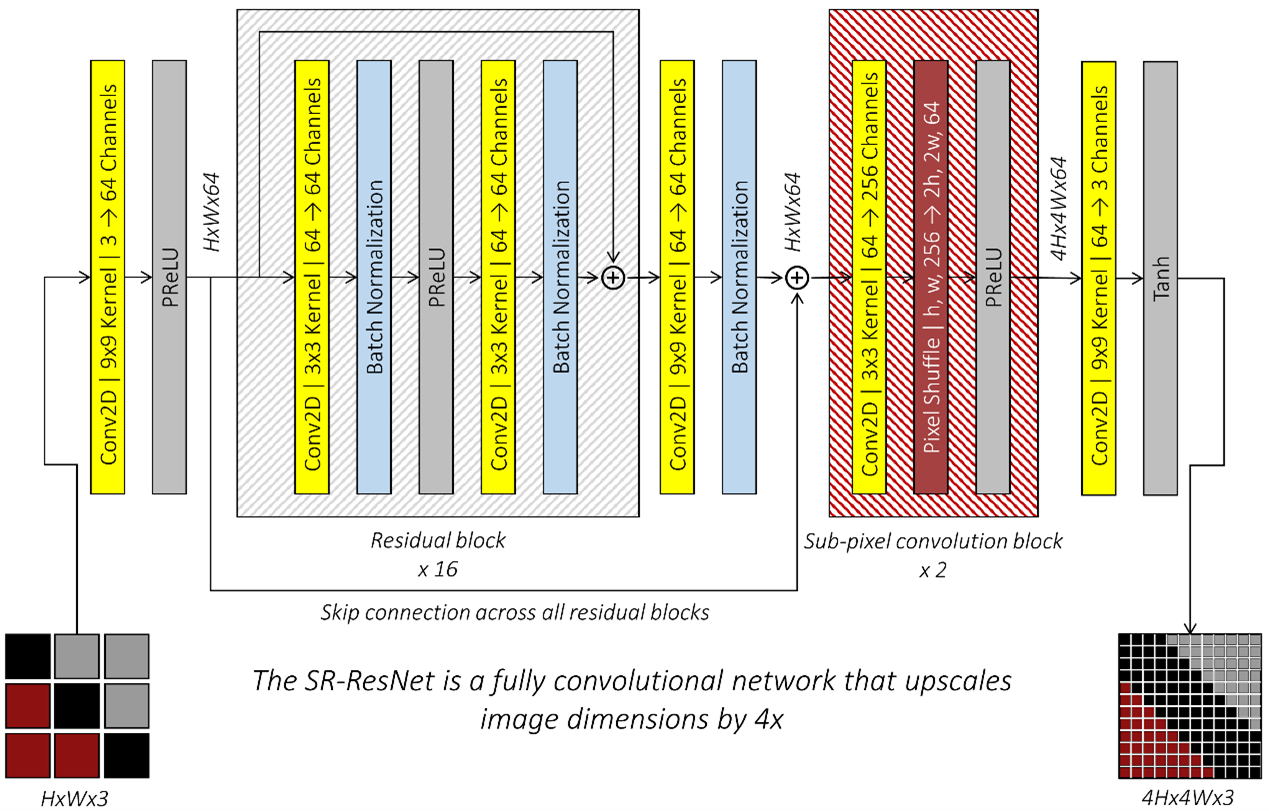
\includegraphics[width=6in]{./figures/srresnet.png}
        \caption{SRResNet Architecture}
    \end{figure}
    The SRResNet first contains convolution block of large Kernel Size 9x9, stride of 1 and 64 channels with PreLU activation. There are 16 residual blocks with convolution layer of Kernel size 3x3 followed by batch normalization, PreLU same conv layer again and batch normalization again. The output then is passed through same 3x3 conv layer and batch normalized. Two subpixel convolution blocks are used followed by PreLU activation each of which provides two times upscaling. Finally, a convolution with large kernel size of 9x9 and 1 stride with 3 out channels for RGB is done with Tanh activation to get super resolved image.\\ In Forward Pass, SRResNet produces a 4x upscaled image from provided low-res image using the above architecture. Mean-Squared Error (MSE) is used as the loss function to compare the upscaled image and original high-quality image. MSE is a type of content loss but here it only looks in RGB space of predicted and target images. Minimizing the MSE by changing the parameters of the network will make the model produce images closer to the original images.

    \end{enumerate}
